\section{State, records and reducers}
\label{sec:records}

\Cref{sec:machines} described the planning agent as an extended state machine, in which a
configuration pairs a control location with the current value of every variable. This section shows
how the runtime stores those values, how one step changes them, and how long each stored value stays
valid. It also separates the stored values from what a model call receives and from what survives
the process, proves that the call budget holds at every step, and shows how the graph is built. The
routing and stopping rules of \cref{sec:routing} read these stored values, so they rest on the
mechanisms described here.

\subsection{State records and schemas}
\label{sec:records-schema}

A \textbf{state record} stores the information that an agent retains between steps as named fields
with their current values. A \textbf{field} is one named entry of the record. \Cref{sec:machines}
called the retained information the state and called its parts variables, so the record is the
stored form of the state and each field holds the value of one variable. For example, the field
\demoref{model\_calls} with the value 2 records that two model calls have completed.

The runtime keeps the control location and the variable values of a configuration in different
places. The runtime itself
tracks the control location, which identifies the computation to run next. The state record holds
the values of the variables, such as the messages exchanged with the model and
\demoref{model\_calls}. The graph of the agent describes control flow, that is, which computation
may run next. The record supplies the values that those computations read.

Each run has its own record, which holds the current values for that run. Every node of the run
reads the same record, so the record is the state that the nodes share.

The fields of the record are declared in a state schema, which, as in Lecture~2, lists the fields
the state contains and their types. Our agents are built with LangGraph, a library for writing
programs as graphs of nodes and edges. LangGraph documents a \demoref{TypedDict} class as the main
way to write a schema \citep{langgraph-graph-api}. A \demoref{TypedDict} is a Python dictionary type
with a fixed set of keys and a declared type for the value of each key \citep{pep589}. Each key of
our schema names one field.

Our schema is the class \demoref{AgentState}. LangGraph builds a graph with its class
\demoref{StateGraph}, and the call \demoref{StateGraph(AgentState)} creates a graph whose shared
state has the fields that \demoref{AgentState} declares.

The schema and the record play different roles. The schema declares the names and types of the
fields, and it is the same for every run. The record holds values, and they change from step to
step. A node never returns a whole record. It returns only the fields that it changes
(\cref{sec:records-updates}). Once those fields are merged into the record, routing functions read
the updated record to select the next node (\cref{sec:routing}).

\subsection{Partial updates}
\label{sec:records-updates}

A node changes the record by returning a partial update, which the runtime merges into the record
one field at a time. A \textbf{partial update} is a mapping from the fields that a node changes to
the values it returns for them.

A \textbf{reducer} is the rule that merges the value stored in a field with the value that a node
returns for that field. Every field has a reducer. A field whose declaration names none takes the
default reducer, which replaces the stored value with the returned one \citep{langgraph-graph-api}.
\Cref{sec:records-reducers} describes the kinds of reducer our agents use.

One step proceeds as follows:
\be
\item The runtime passes the current record, written $s_t$, to the node.
\item While it runs, the node receives an input, written $e_t$: a model reply, a tool result or a
check result.
\item The node returns a partial update, written $u_t$.
\item For each field in $u_t$, the runtime calls that field's reducer. The stored value is the
reducer's left argument, and the returned value is its right argument.
\item The merged record is the next state, $s_{t+1}$.
\ee

\Cref{fig:records-update} draws these steps. The dashed arc carries the stored value from $s_t$
straight to the reducer, so the left argument never passes through the node.

\begin{figure}[htbp]
  \centering
  \begin{adjustbox}{width=\linewidth}
  \begin{tikzpicture}[node distance=6mm and 3mm]
    \node[rnode] (s0) {state $s_t$};
    \node[mnode, right=of s0] (node) {node};
    \node[gnode, right=of node] (upd) {partial\\update $u_t$};
    \node[rnode, right=11mm of upd] (red) {reducer,\\one per field};
    \node[rnode, right=of red] (s1) {state $s_{t+1}$};
    \node[tnode, align=center, below=7mm of node] (ext) {model reply, tool result\\or check result $e_t$};
    \draw[flow] (s0) -- (node);
    \draw[flow] (node) -- (upd);
    \draw[flow] (upd) -- node[lab, below] {right\\argument} (red);
    \draw[flow] (red) -- (s1);
    \draw[flow] (ext) -- (node);
    \draw[back] (s0.north) to[out=35, in=145] node[lab, above] {left argument} (red.north);
  \end{tikzpicture}
  \end{adjustbox}
  \caption{One step of a run. The node reads the stored state and an input, and returns a partial
  update. For each field in the update, the field's reducer merges the stored value (left argument)
  with the returned value (right argument), and the result is the next state.}
  \label{fig:records-update}
\end{figure}

For a field $f$ with reducer $r_f$, where $s_t[f]$ is the value of $f$ in the record $s_t$, the
merge follows one rule:
\begin{equation*}
  s_{t+1}[f] =
  \begin{cases}
    r_f\bigl(s_t[f],\, u_t[f]\bigr) & \text{if } u_t \text{ contains } f,\\[2pt]
    s_t[f] & \text{otherwise.}
  \end{cases}
\end{equation*}
A field omitted from the partial update keeps its stored value. A node therefore never has to copy
the fields it leaves unchanged. It also cannot erase a field by leaving it out.

A node controls only the value it returns. The field's reducer, which the schema declares, fixes how
that value combines with the stored one. The one exception is an explicit overwrite, which bypasses
the reducer (\cref{sec:records-reducers}).

In the terms of \cref{sec:machines}, the partial update and the reducers together carry out the set
action of the transition, the update of the variables. The run then moves to its next control
location, which a routing function selects by reading the merged record (\cref{sec:routing}).

\subsection{The controller's return sites}
\label{sec:records-controller}

The controller ends every visit with a partial update that either stops the run with a status or
records one model call: the reply, the completed call and the reply's token usage. We call each
\demoref{return} statement of a node a \textbf{return site}, and each return site gives the runtime
one partial update. The controller's return sites, in the order its code reaches them, are the
following:
\bi
\item \textbf{Budget.} If the call budget is spent, the controller returns only the field
\demoref{status}, set to \demoref{budget\_exhausted}.
\item \textbf{Stall.} If the stall check finds that the run has stalled, the controller returns only
\demoref{status}, set to \demoref{no\_progress}.
\item \textbf{Model call.} Otherwise, the controller calls the model once. It returns the reply in
\demoref{messages}, one completed call in \demoref{model\_calls}, and the reply's token counts in
\demoref{usage}.
\ei

The first test is the \textbf{admission check}, the comparison of \demoref{model\_calls} with the
budget before each model call (\cref{sec:records-context}). Both stopping tests run before the model
call, so a run that must stop makes no further call. A routing function then reads the status and
ends the run (\cref{sec:routing}).

\Cref{fig:records-controller} applies these return sites to the reactive loop of Lecture~2,
Section~3. Its record is smaller, with ten fields, and its controller has the same return sites in
the same order as the planning agent's. After a model call, the update changes \demoref{messages},
\demoref{model\_calls} and \demoref{usage}. The reducer of \demoref{messages} appends the reply, the
reducer of \demoref{model\_calls} adds one, and the reducer of \demoref{usage} adds each token count
to its running total. A stopping return site changes only \demoref{status}. That field declares no
reducer, so it takes the default, and the returned string replaces the stored one.

\begin{figure*}[t]
  \centering
  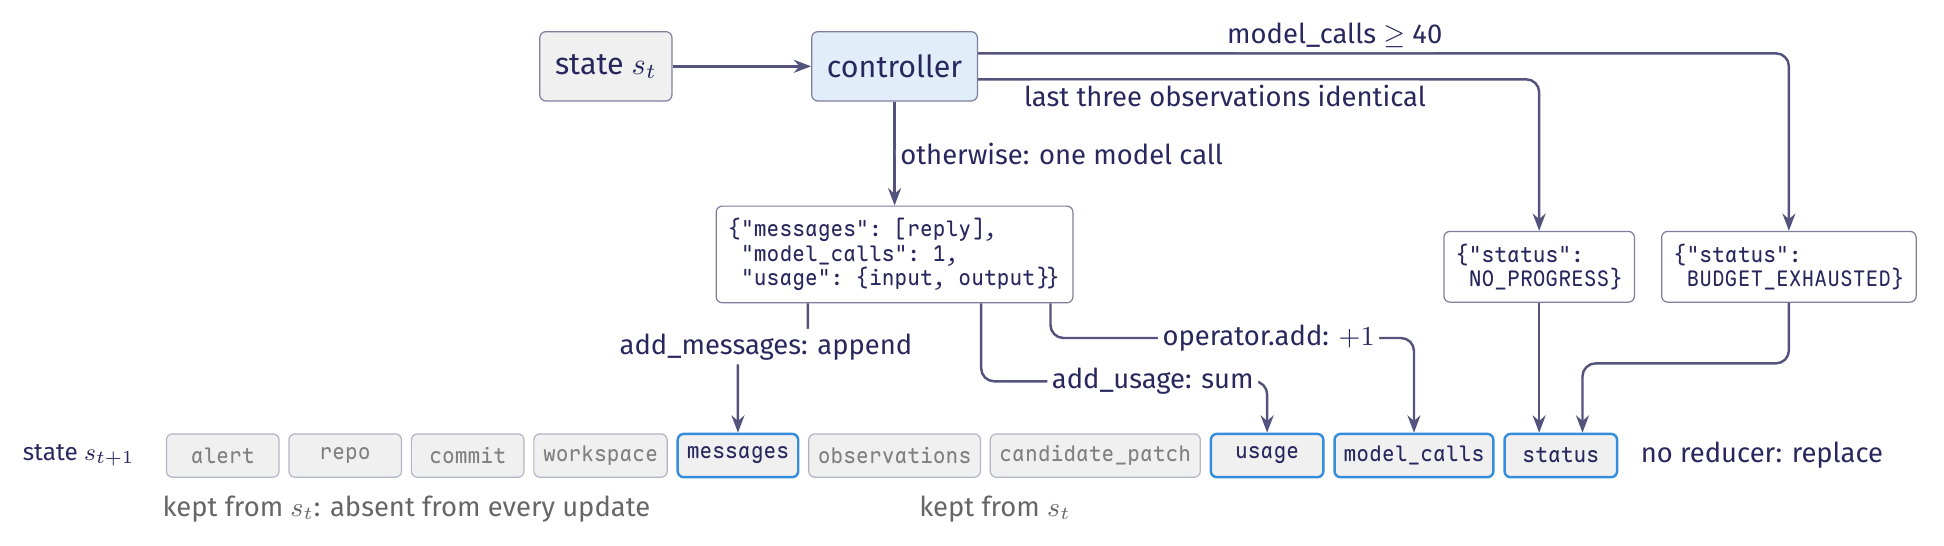
\includegraphics[width=\textwidth]{figures/deck/ee17da9c44.png}
  \caption{The return sites of the reactive loop's controller, applied to its ten-field record. Each
  of the two stopping paths returns only a status. The path through a model call returns the reply,
  one completed call and the reply's token usage (shown with its input and output counts), and each
  of those fields is merged by its reducer. Fields in grey appear in no update and keep their
  stored values.}
  \label{fig:records-controller}
\end{figure*}

The remaining fields, \demoref{alert}, \demoref{repo}, \demoref{commit}, \demoref{workspace},
\demoref{observations} and \demoref{candidate\_patch}, are absent from every update the controller
returns. They keep their stored values after every visit to the controller.

\Cref{lst:records-controller} shows the planning agent's controller. The listing is illustrative and
leaves out the event that the controller writes to the trace.

This controller differs from the reactive loop's in its stall check, which reads only the
observations recorded since the latest revision of the plan, or since the start of the run if the
plan has not been revised. The function \demoref{planning\_window} selects them
(\cref{sec:records-lifetimes}). The tools node detects the first stall and sends the run to the plan
node. In the planning agent, this return site therefore ends the run only when the run stalls again
after a revision.

\noindent\begin{minipage}{\linewidth}
\begin{lstlisting}[basicstyle=\ttfamily\footnotesize, caption={Illustrative code for the planning
agent's controller node. Each \texttt{return} is one return site.}, label=lst:records-controller]
def controller(state):
    stop = admission_check(state)        # budget
    if stop:
        return stop
    if stalled(planning_window(state), limit=3):
        return {"status": NO_PROGRESS}   # stall
    reply = call_model(state["messages"])
    return {"messages": [reply],         # model call
            "model_calls": 1,
            "usage": usage_of(reply)}
\end{lstlisting}
\end{minipage}

The first return site passes on whatever the admission check returns (\cref{lst:records-admission}).
When the budget is spent, the check returns a status update that ends the run. Otherwise it returns
\demoref{None}, and the controller goes on to the stall check.

The second return site applies \demoref{stalled} to the observations that
\demoref{planning\_window} selects. With \demoref{limit=3}, it reports a stall when the last three of
them are identical and none records a successful edit. The last return site reports one completed
call as \demoref{"model\_calls": 1}. The reducer adds this one to the stored count, so a stored count
of 2 becomes 3.

\subsection{Model context, runtime state and durable state}
\label{sec:records-context}

Information about a run exists as model context, runtime state and durable state, which differ in
what they hold, who reads them and how long they last. The \textbf{model context} is what one model
call receives: the instructions, a selection of the history, and observations. Lecture~2 called it
the model's context.

The \textbf{runtime state} is the set of fields that the running process retains between steps,
including counters that the model never sees. It is the state record of \cref{sec:records-schema},
held in the memory of the running process. We say runtime state when we contrast the record with the
model context and the durable state.

The \textbf{durable state} is state that outlives the process, in a form that another process can
load to resume the run. \Cref{tab:records-context} compares the three. Its last column shows the
difference that matters for resuming: only the durable state can be loaded by a new runtime process.

\begin{table}[htbp]
  \caption{Model context, runtime state and durable state: what each holds, and who reads it.}
  \label{tab:records-context}
  \begin{adjustbox}{width=\linewidth}\begin{tabularx}{\linewidth}{L{0.22\linewidth}XL{0.27\linewidth}}
    \toprule
    \textbf{State or context} & \textbf{What it holds} & \textbf{Who reads it} \\
    \midrule
    \textbf{Model context} & The instructions, selected history and observations supplied to one
    model call & The model \\
    \textbf{Runtime state} & The fields retained between steps, including counters that the model
    never sees & Nodes, routing functions and limit checks \\
    \textbf{Durable state} & State that survives the process, in a form another process can load to
    resume the run & A new runtime process \\
    \bottomrule
  \end{tabularx}\end{adjustbox}
\end{table}

For each model call, the runtime builds the model context from the runtime state. The controller
passes the conversation stored in \demoref{messages} to the model (\cref{lst:records-controller}).
The validator's context is built from other fields: the alert, the patch, the check results and
the observations (Lecture~2, Section~4). It never includes the conversation. A model context is
therefore a selection from the runtime state, made separately for each call.

To resume a run after its process exits, the runtime must have saved enough state to reconstruct
the execution. A \textbf{checkpointer} is the component that saves the runtime state as checkpoints
\citep{langgraph-persistence}. Lecture~2 called such saved progress a checkpoint. A checkpointer
that writes its checkpoints to a file or a database produces durable state, which a new process can
load to continue the run. One that keeps them in memory loses them when the process exits. Our
graphs are compiled without a checkpointer and keep their state in memory. When the process exits, the record is lost (\cref{sec:machines}).

The trace survives the process, but a new process cannot rebuild the record from it. The trace
records selected events and omits values that resumption needs, such as the text that each tool
returned, which no event records (\cref{sec:machines}).

A saved record alone is also not enough to resume. The workspace files lie outside the state, so a
resumed run needs files that match the saved record. For example, if the record holds a patch that
was applied before the exit, the files must already contain that patch. A resumed run also needs the
pending work, that is, the steps that were scheduled but had not finished when the process exited.
A later unit of the course covers saved state, pending work and the workspace.

The call budget shows why the distinction between runtime state and model context matters. None of
the planning agent's prompts mentions the budget, so the budget is in no model context. The
admission check enforces it from the runtime state instead (\cref{lst:records-admission}). The
planning agent runs this check before every model call, in each node that calls the model:
\demoref{plan}, \demoref{controller} and \demoref{validate}.

\noindent\begin{minipage}{\linewidth}
\begin{lstlisting}[basicstyle=\ttfamily\footnotesize, caption={Illustrative code for the admission
check, which runs before every model call.}, label=lst:records-admission]
def admission_check(state) -> dict | None:
    if state["model_calls"] >= budget:   # budget = 40
        return {"status": BUDGET_EXHAUSTED}
    return None                          # call allowed
\end{lstlisting}
\end{minipage}

The check works even though the model never receives the budget. It is code in the runtime, and it
compares a counter that the model cannot write with a limit that we fix before the run starts.
Whatever the model writes, a call is issued only while \demoref{model\_calls} is below the budget.

\subsection{Reducers}
\label{sec:records-reducers}

A field's reducer decides how a returned value combines with the stored one, and our agents use
reducers that append, replace or accumulate. The kinds of reducer work as follows:
\bi
\item \textbf{Append.} The reducer adds the returned items to the end of the stored list, so later
nodes can read the full history. The fields \demoref{messages} and \demoref{observations} use append
reducers.
\item \textbf{Replace.} The reducer stores the returned value as the field's new value, as when the
plan node writes a revised plan. A field declared without a reducer takes replacement as its default
\citep{langgraph-graph-api}.
\item \textbf{Accumulate.} The reducer combines the returned contribution with the stored total, for
example by adding 1 to \demoref{model\_calls}. The field \demoref{usage} accumulates token counts in
the same way.
\ei

The schema attaches a reducer to a field with the form \demoref{Annotated[T, fn]}.
\demoref{Annotated} is the standard Python way to attach extra information to a type. Here
\demoref{T} names the field's type, and LangGraph reads \demoref{fn} as the field's reducer
(\cref{lst:records-schema}). A field written with its type alone, such as \demoref{status: str},
declares no reducer and takes the default, which replaces the stored value.

\noindent\begin{minipage}{\linewidth}
\begin{lstlisting}[basicstyle=\ttfamily\footnotesize, caption={Illustrative code for part of the
state schema, with the reducer of each field.}, label=lst:records-schema]
class AgentState(TypedDict, total=False):
    # other fields omitted
    messages: Annotated[list, add_messages]
    observations: Annotated[list, operator.add]
    usage: Annotated[Usage, add_usage]
    model_calls: Annotated[int, operator.add]
    status: str
\end{lstlisting}
\end{minipage}

Each field in the listing has the following reducer:
\bi
\item \textbf{\demoref{messages}.} The reducer \demoref{add\_messages} appends the returned messages
to the conversation. A returned message whose ID matches a stored message replaces that message
instead.
\item \textbf{\demoref{observations}.} The reducer \demoref{operator.add} joins two lists, so it
appends the returned observations.
\item \textbf{\demoref{usage}.} The reducer \demoref{add\_usage} accumulates. It keeps four separate
token counters and adds each returned count to the counter of the same kind. One counter holds cache
reads, the input tokens that the provider reuses from an earlier call, so they stay distinct from
fresh input tokens.
\item \textbf{\demoref{model\_calls}.} The same \demoref{operator.add} adds two integers here, so it
accumulates the count of completed calls.
\item \textbf{\demoref{status}.} The field declares no reducer, so it takes the default, and an
update replaces the stored string. If a node returns no status, the runtime keeps the previous one.
\ei
The words \demoref{total=False} in the class header declare that a dictionary of this type may
leave keys out \citep{pep589}. A partial update, which holds only some of the keys, therefore still
has the declared type.

Returning \demoref{[]} to an append reducer adds zero items, so the stored list keeps its contents.
Clearing a list such as \demoref{observations} therefore requires an explicit overwrite, which
bypasses the reducer and replaces the stored value.

LangGraph provides the wrapper \demoref{Overwrite} for this. A node that returns a value wrapped in
\demoref{Overwrite} replaces the stored list with that value. A reset of this kind should be
recorded as its own trace event. A reader of the trace otherwise assumes that the list only grows,
and cannot tell that earlier entries were discarded.

\subsection{Field lifetimes}
\label{sec:records-lifetimes}

A \textbf{field lifetime} is the interval during which later nodes may rely on a field's stored
value. The lifetime ends when a later step makes that value obsolete, for example when a revision of
the plan makes the old plan obsolete. A reducer decides only how a returned value is merged. It does
not decide how long later nodes may rely on that value.

\Cref{tab:records-lifetimes} defines the lifetimes. In our two agents, the identity fields are
\demoref{alert}, \demoref{repo}, \demoref{commit} and \demoref{workspace}. The run fields are
\demoref{messages}, \demoref{observations}, \demoref{usage} and \demoref{model\_calls}. The current
fields are \demoref{candidate\_patch}, \demoref{status}, \demoref{plan}, \demoref{checks} and
\demoref{validation}.

A \textbf{handoff field} holds a reason that one node leaves for another and is cleared after use,
here \demoref{failed\_step}. A \textbf{window field} holds an index where a window of a history
starts, here \demoref{replanned\_at}. An attempt is one try at producing an accepted patch. No field
of either agent has the attempt lifetime.

\Cref{fig:records-schemas} sets the two schemas side by side. The shading of each field gives its
lifetime from \cref{tab:records-lifetimes}, and a plus sign marks the fields that the planning agent
adds: \demoref{plan}, \demoref{failed\_step}, \demoref{replanned\_at}, \demoref{checks} and
\demoref{validation}.

The plan node writes \demoref{plan}, the submit node writes \demoref{checks}, and the validate node
writes \demoref{validation}. Each of these fields holds the latest value until its writer replaces
it. The tools node writes \demoref{failed\_step} for the plan node to read and clear. The index
\demoref{replanned\_at} marks where the observations made under the current plan begin.

\begin{figure*}[t]
  \centering
  \definecolor{recordslifeid}{HTML}{E4E4E4}
  \definecolor{recordsliferun}{HTML}{D0E2FF}
  \definecolor{recordslifecur}{HTML}{D4F0D4}
  \definecolor{recordslifehand}{HTML}{FFDFB8}
  \definecolor{recordslifewin}{HTML}{E6D6FF}
  \newcommand{\recordslf}[3][]{\par\noindent\hspace*{1em}\llap{\textbf{#1}\hspace{0.3em}}%
    {\setlength{\fboxsep}{0.6pt}\colorbox{#2}{\makebox[\dimexpr\linewidth-1em-1.2pt][l]%
    {\ttfamily\strut\hspace{1.5em}#3}}}\par}
  \newcommand{\recordslfhead}[1]{\par\noindent\hspace{1em}{\ttfamily\strut#1}\par}
  \newcommand{\recordslfgap}{\par\vspace{2pt}}
  \newcommand{\recordslfcap}[1]{\par\noindent{\sffamily\bfseries #1}\par\smallskip}
  \newcommand{\recordslfkey}[2]{{\setlength{\fboxsep}{1.5pt}\colorbox{#1}{#2}}}
  \setlength{\parskip}{0pt}%
  \footnotesize
  \begin{minipage}[t]{0.47\textwidth}
    \recordslfcap{The reactive loop}
    \recordslfhead{class AgentState(TypedDict, total=False):}
    \recordslf{recordslifeid}{alert: dict}
    \recordslf{recordslifeid}{repo: str}
    \recordslf{recordslifeid}{commit: str}
    \recordslf{recordslifeid}{workspace: str}
    \recordslfgap
    \recordslf{recordsliferun}{messages: Annotated[list, add\_messages]}
    \recordslf{recordsliferun}{observations: Annotated[list, operator.add]}
    \recordslf{recordslifecur}{candidate\_patch: str | None}
    \recordslf{recordsliferun}{usage: Annotated[Usage, add\_usage]}
    \recordslf{recordsliferun}{model\_calls: Annotated[int, operator.add]}
    \recordslf{recordslifecur}{status: str}
  \end{minipage}\hfill
  \begin{minipage}[t]{0.47\textwidth}
    \recordslfcap{The planning agent}
    \recordslfhead{class AgentState(TypedDict, total=False):}
    \recordslf{recordslifeid}{alert: dict}
    \recordslf{recordslifeid}{repo: str}
    \recordslf{recordslifeid}{commit: str}
    \recordslf{recordslifeid}{workspace: str}
    \recordslfgap
    \recordslf[+]{recordslifecur}{plan: list | None}
    \recordslf[+]{recordslifehand}{failed\_step: dict | None}
    \recordslf[+]{recordslifewin}{replanned\_at: int}
    \recordslf{recordsliferun}{messages: Annotated[list, add\_messages]}
    \recordslf{recordsliferun}{observations: Annotated[list, operator.add]}
    \recordslf{recordslifecur}{candidate\_patch: str | None}
    \recordslf[+]{recordslifecur}{checks: dict | None}
    \recordslf[+]{recordslifecur}{validation: dict | None}
    \recordslf{recordsliferun}{usage: Annotated[Usage, add\_usage]}
    \recordslf{recordsliferun}{model\_calls: Annotated[int, operator.add]}
    \recordslf{recordslifecur}{status: str}
  \end{minipage}

  \medskip
  {\sffamily Lifetime:\enspace
  \recordslfkey{recordslifeid}{identity}\enspace\recordslfkey{recordsliferun}{run}\enspace
  \recordslfkey{recordslifecur}{current}\enspace\recordslfkey{recordslifehand}{handoff}\enspace
  \recordslfkey{recordslifewin}{window}\qquad\textbf{+}\,new in the planning agent}
  \caption{The state schemas of the reactive loop and the planning agent. The shading of each field
  gives its lifetime, and a plus sign marks the fields that the planning agent adds.}
  \label{fig:records-schemas}
\end{figure*}

\begin{table}[htbp]
  \caption{The field lifetimes, with what each one means for the nodes that read and write the
  field.}
  \label{tab:records-lifetimes}
  \begin{adjustbox}{width=\linewidth}\begin{tabularx}{\linewidth}{L{0.2\linewidth}X}
    \toprule
    \textbf{Lifetime} & \textbf{Definition and use} \\
    \midrule
    \textbf{Identity} & Identity fields identify the task, the target and the workspace, and they
    remain unchanged. \\
    \textbf{Run} & Run fields retain histories and counters that grow throughout the run. \\
    \textbf{Current} & Current fields hold the latest plan, candidate, check result or status until
    the writer replaces them. \\
    \textbf{Handoff} & One node writes a reason for invoking another node. The receiving node reads
    that handoff field and clears it after acting. \\
    \textbf{Window} & An index field marks where a selected window of history begins. Checks read
    from that index onward while the complete history remains stored. \\
    \textbf{Attempt} & An attempt field holds the results of one attempt. Nodes clear it before a
    new attempt, so later steps cannot treat old results as current. \\
    \bottomrule
  \end{tabularx}\end{adjustbox}
\end{table}

The attempt lifetime is absent because neither agent starts a new attempt. In the planning agent,
a rejection by the validator ends the run, and the reactive loop has no validator. In both agents, a
patch that fails the checks returns to the controller for repair, but no field is cleared, and the
run continues as a single attempt. Neither schema
therefore needs fields that must be cleared before a new attempt.

\Cref{sec:routing} discusses a proposed new attempt after a rejection. If it were added, fields that
hold one attempt's results, such as the plan and the candidate patch, would become attempt fields.

The runtime merges updates according to reducers. It does not enforce lifetimes, so node code
must enforce them, by retaining, replacing or clearing each field when required. A reducer sees
only the stored value and the returned value. It cannot know that a revision has happened or that
a reason has been acted on.

Run fields must keep their values across attempts, which matters once a new attempt is added
(\cref{sec:routing}). The call count shows why. A counter that limits the whole run must keep its
total. If \demoref{model\_calls} were reset to zero at a new attempt, later calls would ignore the
calls already spent, and the budget would no longer bound the run. Attempt fields are the opposite
case. They would be cleared before a new attempt because their old results no longer apply.

The handoff field and the window field of the planning agent work together when the run stalls
(\cref{lst:records-handoff}). When the tools node detects the first stall, it stores the reason in
\demoref{failed\_step}. The plan node uses that reason to revise the plan, then clears
\demoref{failed\_step} and sets \demoref{replanned\_at}.

\begin{lstlisting}[float=tbp, basicstyle=\ttfamily\footnotesize, caption={Illustrative excerpts from the tools
node and the plan node: the handoff in \texttt{failed\_step} and the window in
\texttt{replanned\_at}.}, label=lst:records-handoff]
# tools node: hand off to plan on the first stall
update = {"observations": new}  # tool messages omitted
window = state["observations"] + new  # not merged yet
if (not state.get("replanned_at")
        and stalled(window, limit=3)):
    update["failed_step"] = {...}   # the reason
# plan node: revise, clear the handoff, open a window
# (the admission check that runs first is omitted)
failed = state.get("failed_step")
steps = call_planner(state, failed)   # one model call
update = {"plan": steps, "failed_step": None,
          "model_calls": 1}   # messages, usage omitted
if failed:
    update["replanned_at"] = len(state["observations"])
\end{lstlisting}

The tools node tests the stored observations together with its new ones, because the runtime merges
its update only after the node returns (\cref{sec:records-updates}). Its update always holds the new
observations, and it gains \demoref{failed\_step} only on the first stall.

Clearing \demoref{failed\_step} removes the request for the revision just completed. If the field
remained set, the routing function after the tools node, \demoref{after\_tools}, would select the
plan node again on the next tools step. The test \demoref{not state.get("replanned\_at")} also
limits the handoff to one revision, because the index is set once the plan has been revised.

The plan node sets \demoref{replanned\_at} to the number of observations stored when the revision
completes. The slice \demoref{observations[replanned\_at:]} therefore starts with the observations
made under the revised plan. The stall check reads only this window, while the earlier observations
remain in the full history. Lecture~2 called \demoref{replanned\_at} a high-water mark.

A window field lets a check ignore old entries of a run field without clearing that field. The list
\demoref{observations} has an append reducer, so clearing it would need an explicit overwrite
(\cref{sec:records-reducers}). It would also remove evidence that later nodes read, such as the
validator, which judges the patch from the observations.

\subsection{The call budget as an invariant}
\label{sec:records-invariant}

The call budget bounds the number of completed model calls because a property of the record holds
at every step. An \textbf{invariant} is a property that holds in every reachable configuration of a
machine. The standard proof first shows that the property holds in the initial configuration. It
then shows that every transition from a configuration where the property holds leads to a
configuration where it still holds. The property then holds in every configuration that a run can
reach \citep[Theorem~2, p.~5]{mit6042-lec16}.

The invariant of the call budget is that \demoref{model\_calls} counts the completed model calls
exactly and never exceeds the budget $B$, which is 40 in our agent:
\begin{equation*}
  \text{\ttfamily model\_calls} = \text{number of completed model calls} \le B.
\end{equation*}
In the initial configuration, \demoref{model\_calls} is 0 and no call has completed. The argument
that every transition keeps the property true covers steps that call the model (admission and
counting) and steps that do not (preservation):
\bi
\item \textbf{Admission.} Each node that calls the model checks that the stored call count is
below the budget before it issues the call. A call therefore starts only when the count is at
most $B-1$.
\item \textbf{Counting.} After a call completes, the node returns \demoref{"model\_calls": 1}, and
the reducer adds one to the stored count. The count rises by one for each completed call, and
because the call started at $B-1$ or less, the count reaches at most $B$.
\item \textbf{Preservation.} A step without a model call leaves the count unchanged, because the
field is absent from its partial update. No transition resets or decreases the count.
\ei

The reducer only accumulates the calls that nodes report. The property therefore depends on every
caller. Each node must check the budget before calling and must report each completed call exactly
once. A node that called the model without the admission check, or reported a call twice, would
break the invariant, and the reducer could not detect it.

The argument covers completed calls only. A call that is interrupted, for example because the
process is stopped while the call is in progress, may consume tokens without being counted. Its
node never returns an update, so \demoref{model\_calls} never includes it. The invariant bounds the
completed calls of a run. It does not bound everything the run spent. \Cref{sec:routing} uses the
budget to argue that a run ends.

\subsection{Building and compiling the graph}
\label{sec:records-compile}

The graph is built by declaring its schema, its nodes and its edges, and then compiling the
declarations into a graph that the runtime can execute (\cref{lst:records-compile}). The call
\demoref{StateGraph(AgentState)} creates one \textbf{channel} per field of the schema. A channel is
the runtime's store for one field. It holds the field's value and applies each update with the
field's reducer. For a field that declares no reducer, the channel replaces the stored value, as the
default reducer does \citep{langgraph-pregel}.

\noindent\begin{minipage}{\linewidth}
\begin{lstlisting}[basicstyle=\ttfamily\footnotesize, caption={Illustrative code that builds and
compiles the planning agent's graph, with most declarations omitted.}, label=lst:records-compile]
graph = StateGraph(AgentState)   # one channel per field
graph.add_node("plan", plan)
graph.add_node("tools", tools)
# other nodes and edges omitted
graph.add_edge(START, "plan")
graph.add_conditional_edges("tools", after_tools,
    {"controller": "controller", "plan": "plan"})
graph.add_edge("validate", END)
app = graph.compile()
\end{lstlisting}
\end{minipage}

The declarations do the following:
\bi
\item \textbf{\demoref{add\_node}.} It associates a node name with the function that the runtime
will call for that node. The function receives the state and returns a partial update.
\item \textbf{\demoref{add\_edge}.} It names the node that always runs after a source node
finishes. The edge from \demoref{START} begins every run at the plan node, and the edge to
\demoref{END} ends the run after the validator.
\item \textbf{\demoref{add\_conditional\_edges}.} It attaches a routing function to a source node,
together with a mapping from each value the function can return to the node that runs next. After
the source node's update is merged, the runtime calls the routing function, which reads the updated
record and selects one of these successors. After the tools node, the destination is the plan node
after the first stall, and the controller otherwise.
\item \textbf{\demoref{compile}.} It checks the declared connections of the graph and returns a
graph that the runtime can execute.
\ei

The runtime fixes the order of operations in a step. The node runs and returns its update, the
channels merge it, and only then does a routing function read the record. A routing decision
therefore always sees the values that the node just returned.

\subsection{Designing a state graph}
\label{sec:records-design}

A \textbf{state graph} is a graph whose nodes read and update one shared state record, like the one
built in \cref{sec:records-compile}. We design one by declaring each field at the same time as the
node that writes it, in the following steps:
\be
\item \textbf{Specify the nodes} and the rules that select which node runs next.
\item \textbf{Declare fields} for the values that nodes and routing functions read.
\item \textbf{Name the node} that writes each field, and say when later nodes must stop using its
old value.
\item \textbf{Choose each field's lifetime,} and then choose whether its updates append, replace or
accumulate values.
\item \textbf{Write the initial record} with a value for every field.
\item \textbf{Make each node} return a partial update that contains only the fields it proposes to
update.
\ee

The field \demoref{failed\_step} of the planning agent shows the steps applied to one field. The
plan node and the routing function after tools read it, so it is declared. The tools node writes
it, and its value is obsolete once the plan node has revised the plan. Its lifetime is therefore a
handoff, and its update replaces the stored value.

The initial value of \demoref{failed\_step} is \demoref{None}. When the tools node detects the first
stall, it adds the field to the partial update that already holds its new observations and messages,
and it leaves every other field out of that update. The plan node returns \demoref{None} for the
field once the revision is done.

Each field retains a value that a later computation needs to read. A field that no computation
reads should be left out of the schema.

\subsection*{Key points}
\bi
\item A state record stores the information an agent retains between steps as named fields, the
runtime tracks the control location separately, and the schema declares the fields' names, types
and reducers.
\item A node returns a partial update, each returned field's reducer merges the stored value (left
argument) with the returned value (right argument), an omitted field keeps its value, and routing
then reads the merged record.
\item In order, the controller's return sites give the status \demoref{budget\_exhausted} when the
budget is spent, the status \demoref{no\_progress} when the run has stalled, and otherwise the reply,
one completed call and its token usage.
\item The model context is the part of the runtime state selected for one model call, and the
durable state is what a checkpointer saves to a file or a database so that another process can
resume the run.
\item A reducer appends, replaces or accumulates, and since returning an empty list to an append
reducer adds nothing, clearing a list such as \demoref{observations} needs an explicit overwrite,
recorded as its own trace event.
\item A field's lifetime is the interval in which later nodes may rely on its value, and node code
must enforce it, as the plan node does when it clears the handoff field \demoref{failed\_step} and
sets the window field \demoref{replanned\_at}.
\item Because each node that calls the model runs the admission check before the call and reports
each completed call once, \demoref{model\_calls} never exceeds the budget, which no model context
contains, but the bound covers completed calls only, and an interrupted call can consume tokens
without being counted.
\ei
